\documentclass[11pt]{article}   % list options between brackets
              % list packages between braces
\usepackage{geometry}

\usepackage{algorithm}
\usepackage[noend]{algpseudocode}

\usepackage[pdftex]{graphicx}
\geometry{verbose,a4paper,tmargin=15mm,bmargin=30mm,lmargin=30mm,rmargin=20mm}
\usepackage{graphics}
% type user-defined commands here

\begin{document}
\begin{titlepage}
\thispagestyle{empty}
\vspace*{0.7cm}
{\centering     
\large
{\huge\bf Slicing of \\}\emph{ Web Applications using Source Code Analysis}\\
\vspace{2.5 cm}
\emph{Synopsis report submitted in partial fulfilment\\
of the requirements for the degree of}\\
\vspace{1 cm}{ \bf \large Bachelor of Technology}\\
\emph{in}\\
\bf Computer Science and Engineering\\

\vspace{1cm}
\it
by \\
\vspace{.5cm}
\rm
{\large \bf {Ankit Kumar and Anubhav Panda}}\\
{\large \bf {111CS0129 and 111CS0044}}

\vspace{1cm}

{\it{under the guidance of}} \\
\vspace{.5cm}

\hspace{.05cm} {\large \bf {Prof. D.P.Mohapatra}}\\
\hspace{.05cm} 
\vspace {0.5cm}
\vspace {1 cm}
%\iitbseal\ \\

\begin{figure}[h] 
%\hspace{3cm}
%\vspace{3cm}
\centering
%\includegraphics{images.jpg}
\end{figure} 

Department of Computer Science \& Engineering \\ 
National Institute of Technology, Rourkela\\ Rourkela-769008, Odisha, INDIA\\
{\centering
\hspace{6.5cm}March, 2015} 
}
\pagebreak 
\end{titlepage}
\newpage
\begin{minipage}[t]{.2\textwidth}
\vspace{0pt}
\includegraphics[width=3cm,height=3cm]{./nit.png}
\end{minipage}%
\hspace{10pt}
\begin{minipage}[t]{.8\textwidth}
\vspace{30pt}
\break
 Department of Computer Science and Engineering\\
\textbf{National Institute of Technology, Rourkela}\\
Rourkela-769008, Odisha, India
\begin{flushright}
\today\\
\end{flushright}

\end{minipage}

\vspace{1cm}
\begin{center}
\begin{Large}
\textbf{Certificate}
\end{Large}
\end{center}

This is to certify that the work in the thesis entitled \emph{ Slicing of Web Applications using Source Code Analysis} by Anubhav Panda and Ankit Kumar is a record of an original research work carried out under my supervision and guidance in partial fulfillment of the requirements for the award of the degree of Bachelor of
Technology in Computer Science and Engineering. Neither this thesis nor any part of it has been submitted for any degree or academic award elsewhere.

\vspace{2cm}

\begin{flushleft}
Durga Prasad Mohapatra\\
Associate Professor,\\
Dept of Computer Science and Engineering,\\
NIT Rourkela
\end{flushleft}

\large
\small
\newpage
\pagenumbering{roman}
\begin{abstract}
%\boldmath
Program slicing revealed a useful way to limit the search of software defects during debugging and to better understand the decomposition of the application into computations. The web application is very widely used for spreading business through out the world. To meet the desire of the customers, web applications should have more quality and robustness. Slicing, in the field of web application, helps disclosing relevant information and understanding the internal system structure. This in-terns help in debugging, testing and in improving the program comprehensibility.

The system dependence graph is an appropriate data structure for slice computation, in that it explicitly represents all dependencies that have to be taken into account in slice determination. We have extended the system dependence graph to Web-Application Dependence Graph (WADG). We have developed a partial tool for automatic generation of the WADG and computation of slices. In our literature survey, we found that most of the automatic graph generation tools are byte-code based. But, our tool uses the dependency analysis form the source code of the given program. We have presented three case studies by taking open source web programs and applying our techniques and slicing algorithm. We have found that the slices computed is correct and precise, which will be help full for program debugging and testing.
\par Construction of the system dependence graph for Web applications is complicated by the presence of dynamic code. In fact, a Web application builds the HTML code to be transmitted to the browser at run
time. Knowledge of such code is essential for slicing

\end{abstract}

\newpage
\pagenumbering{roman}

\thispagestyle{empty}
\tableofcontents

\newpage



\pagenumbering{arabic}

\section{Introduction}
\par One of the first systematic studies on Web site analysis is, where the evolution of the entities in Web sites is characterized by means of a set of metrics traced over time.
Program slicing is a special type of static analysis, consisting of a decomposition technique for the extraction of program statements relevant to a specified computation. Program slicing has many applications such as debugging, code understanding, program testing, reverse engineering, software maintenance, reuse, software safety and metrics. A Web application consists of a set of Web pages displayed to the user and of a set of server side programs (usually scripts), performing some computation and producing output pages to be displayed.
\par Java Server Pages (JSP) web applications focuses more on presentation logic. They are easier to maintain than a servlet. As opposite to servlets, JSP adds Java code inside HTML rather than adding HTML code inside Java code but can still achieve everything that a servlet can do.
\par We will present an approach to Web application slicing. A Web application is a special case of client-server system, in which the Web server plays the role of the server,the Web browser plays the role of the client which establishes communication between the client and the server by using some specific protocols (http, https). Due to the process of modularization most of the current applications use the service of web servers or web APIs (Application Programming Interfaces). With the development of internet the quality of web applications has also increased and is continuing to do so. The result of slicing a Web application is still a Web application (often simpler than the initial one), which exhibits the same behavior as the initial Web application with respect to some information of interest. Web application slicing can be used, as with traditional software systems, to assist programmers and Web designers in tedious and error prone tasks such as understanding, debugging, and regression testing \cite{tsai2001scenario}\cite{masri2004detecting}\cite{xu2003regression}.\cite{wu2004slicing}
\par In this thesis we have proposed our approach to handle the web pages which consists of JSP ,HTML and JavaScript parts. We have processed the 3 parts differently and generated the WADG (Web Application Dependence Graph) in order to explain the flow of web applications  as well as different kind of dependence between them. We have considered page call and function call differently. Also, we have applied our slicing algorithm upon the generated WADG with multiple Slicing criteria and analyzed the resulting slices.We are also working on the dynamic slicing of web application. And we have considered different cases of  it.
\par Web applications comprising dynamically generated pages are  more difficult
to analyze than staticWeb sites. The server script that is executed when a page is requested
builds the HTML structure of the resulting page at run time. The tags inserted into the
page can, in general, depend on the state of the program and on the input values or the value from the databases. Moreover, even the names of the HTML variables in the generated page, the FORM, ACTIONS and
the hyperlinks can be constructed dynamically, and vary from execution to execution. If
the WADG is constructed with no regard to the generated code, important nodes and edges
are possibly missed. For example, when tags are produced dynamically, the related nodes
are not in the WADG built for the server script. When variable names are generated dynamically,
the data dependences associated to them are absent in the WADG. When FORM,ACTIONS
are inserted dynamically in a page, the related call dependences are not reported in the WADG.
The problem of statically constructing a precise WADG for a dynamicWeb application is in
general undecidable. This means that there existWeb applications for which it is not possible
to build a precise WADG just by analyzing the source code, because the dynamically generated
WADG nodes cannot be approximated statically. However, under reasonable assumptions it
is possible to devise static analysis techniques that are able to precisely produce the WADG
for a subset of all possibleWeb applications, including most of the real world ones. 
Another completely different approach to the problem of determining the dynamically
constructed WADG portions relies on dynamic slicing. When a specific execution of a Web
application is considered, with given input values, the problem of approximating the generated
HTML code disappears, since this can be obtained by actually running the application.
Thus, slices can be computed directly on the generated code, which is known. However, the
resulting slices hold only for the input values used in the execution. Some of the excluded
portions of the Web application could be relevant to the selected computation for different
inputs. This is why we focus on static slicing.We are currently working on static construction of the WADG for Web
applications in presence of dynamic code generation. The code produced at run time is
“extruded” from the statements that generate it. However, code extrusion is not sufficient
when the generated code is accumulated into a string variable before being printed out. A
flow analysis algorithm, called string-cat propagation, is proposed to handle such cases.
Combined with code extrusion, it allows treating several programming patterns commonly
used withWeb applications, such as string variables, where the HTML code is temporarily
stored, and general purpose functions, that are parameterized at invocation in order to
generate the desired HTML fragment.
%\hfill mds
\section{Basic concepts}
A program slice is a reduced, executable program obtained from a given program by removing statements, so that it replicates part of the behavior of the initial program.\cite{Weiser}\cite{weiser1981program}\\
Similar concept has been applied on web applications to generate web application slicing. This can be achieved with the help of system dependence graph.

\subsection{Web Slicing}
A Web application consists of a set of Web pages displayed to the user and of a set of server side programs (usually scripts), performing some computation and producing output pages to be displayed. As a consequence, slicing a Web application should result in a Web application which exhibits the same behavior as the initial Web application with respect to the information of interest.
 A Web application slice is obtained from a given set of Web pages and scripts by selecting HTML and script statements, so that part of the behavior of the initial Web application is replicated.\cite{ricca2001web}\cite{mao2009slicing}


\subsubsection{Slicing Criterion}
The criterion for slice computation is an information item of interest displayed in a given Web page, and the resulting slice reproduces the same information item, if the user performs the same navigation actions and provides the same input in the original and in the sliced Web application. Formally, a slicing criterion (n, x) consists of a statement n, displaying the information item of interest, and a variable x, used for the production of such an information item\cite{ricca2001web}.
\subsubsection{Types of Slicing}
There are many types of program slicing exists. Slicing can be distinguished by the nature of program's execution or by its approach. We are here presenting some basic types of slicing, but for more detailed study some good review papers \cite{Binkley}\cite{de2001program}, can be referred.

\emph{Static Slicing}:
A static slice includes all the statements that affect variable v for a set of all possible inputs at the point of interest (i.e., at the statement x). Static slices are computed by finding consecutive sets of indirectly relevant statements, according to data and control dependencies.

\emph{Dynamic Slicing}:
A dynamic slice contains all statements that actually affect the value of a variable at a program point for a particular execution of the program rather than all statements that may have affected the value of a variable at a program point for any arbitrary execution of the program.

\emph{Forward Slicing}:
Forward slice consists of all statements and control predicates dependent on the slicing criterion, a statement being "dependent" on the slicing criterion if the values computed at that statement depend on the values computed at the slicing criterion, or if the values computed at the slicing criterion determine the fact if the statement under consideration is executed or not.

\emph{Backward Slicing}:
A backward slice contains statements of a program which has some effect on the slicing criterion. It helps the developer to locate the parts of the program that contains a bug. Backward slice requires tracing dependencies in the backward direction.

\subsection{System Dependence Graph}
A System Dependence Graph (SDG) is used to model dependence between statements within a procedure including inter-procedural dependence. The final slicing algorithm will be depend over the SDG. 
The SDG is a graph whose nodes roughly correspond to program statements and whose edges model dependence in the program.

There are various types of dependence which could explain the different relation between two statements of the input program.
\subsubsection{Control Dependence}
A control dependence holds between two statements if the former defines a scope which directly includes the latter. It is also known as nested dependence.
Control dependence for traditional programs connect the predicate tested at a conditional or loop statement to the instructions the execution of which directly depends on the truth value of the predicate. The same holds for the server side scripts, but Web applications are also characterized by an additional kind of control dependence, which is found in the HTML code between a tag and all directly enclosed statements\cite{ricca2001web}.
\subsubsection{Data Dependence}
A data dependence holds between two server side statements or between a server side and an HTML statement if the former defines the value of a variable which is used by the latter, and a definition clear (i.e., a path containing no redefinition of the given variable) path exists between the two.
Data dependence for traditional programs are associated with statements defining the value of a variable, which is used at another statement after being propagated to it along a definition clear path.\cite{ricca2001web}
\subsubsection{Call Dependence}
A call dependence holds between each HTML input statement of type submit and the dynamic page specified in the associated action.
When a server side program is invoked from an HTML statement (e.g., via form submission or HREF), control of execution is transferred to the server and never returns back to the Web page issuing the call. In other words, a server program invoked from an HTML statement cannot produce any effect on the variables of the calling page, since the invocation is a no-return invocation. A consequence is that the calling context problem, i.e., the problem of keeping the data flows associated to the different call sites separated, is absent, since call sites are not affected by the invocation\cite{ricca2001web}.
\subsubsection{Parameter - In}
A parameter-in dependence holds between an HTML input statement and a server side request-form statement if the form containing the input calls the dynamic page containing the request form and the names of input and requested variables are the same\cite{ricca2001web}.
\subsubsection{Parameter - Out}
A parameter-out dependence holds between any value returned from an invocation and the related variable in the call site.
\subsubsection{Summary Edge}
In the case of slicing, summary edges represent a transitive data dependence through a particular call
site. Summary edges connect actual-in vertices with actual-out vertices and represent a that dependence
between the connected vertices may be created in the called procedure/pages or (transitively) through other called
procedures/pages.
\subsection{Web Application Dependence Graph}
A System Dependence Graph is incapable of handling web applications and is only suitable for programs. Hence we introduce a Web Application Dependence Graph(WADG) with following additional dependences:-
\subsubsection{Event Loop}
Mouse or keyboard events occurring during or after page loading can trigger the execution of a client side procedure, can produce the loading of another page (hyperlinks), or the calling of a JavaScript. The graphical user interface of the browser handles such events by means of a so called event loop.
\subsubsection{PageCall Dependence}
A PageCall dependence holds between each HTML input statement of type submit and the dynamic page specified in the associated action.
\subsubsection{Build Dependence}
A build dependence holds between a server program statement and an HTML statement if the former generates the latter.
During slice computation, build dependences are traversed backward similarly to the other dependences. In this way, the statements in the original program responsible for generating the HTML statements included in the slice will be also part of the slice.\cite{tonella2005web}
\begin{figure}
\begin{center}
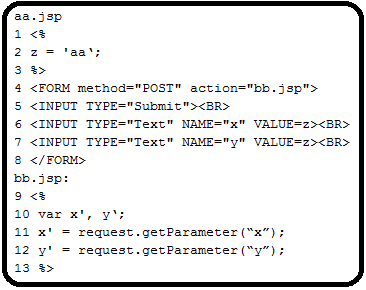
\includegraphics[scale=1.3]{example.png}
\end{center}
\caption{Sample JSP program }
\label{fig1}
\end{figure}
\begin{figure}

\begin{center}
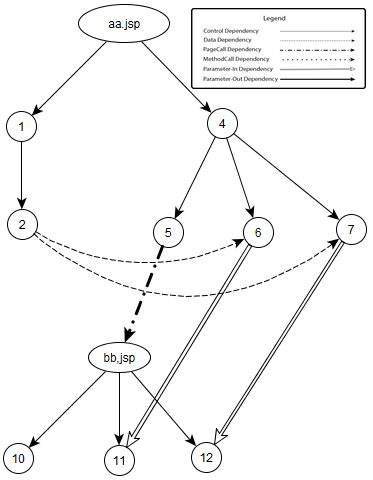
\includegraphics[scale=0.8]{SDG_example_l.png}
\end{center}
\caption{SDG of the program in fig-\ref{fig1} }
\label{fig2}
\end{figure}
\\\\
In the above example (in Figure-\ref{fig1}), the first jsp page consists of two subsections of code, i.e, HTML and Java beginning at statements 1 and 4 respectively. Thus, there is a control dependence between the page name and the two statements. Similarly, there is a control dependence between statement 1 and all other Java statements, i.e 1 and also between statement 4 and all other HTML statements, i.e,5,6,7 enclosed within tag represented by statement 4.

Now, statements 6 and 7 get their value of x from statement 2, resulting in data dependence between statement 2 to 6 and 2 to 7.

Also, the page bb.jsp is called when the FORM in aa.jsp is submitted from click event of statement 5, resulting in a call dependence between statement 5 and bb.jsp.
Values are passed from statement 6 to 11 and statement 7 to 12 resulting in a parameter-in dependence between those statements. The final SDG for the above example program is shown in Figure-\ref{fig2}.
 
\section{Related Works}
In this section, we present a brief survey of the existing literatures those are closely related to our work.

\subsection{Slicing of Web Applications}
\par A web application consists of, a set of web pages displayed to the user and a set of server side programs (usually scripts). The web application performs some computation and produces output pages to be displayed. A web application slice is obtained from a given set of web pages and scripts, by removing HTML and script statements, so that part of the behavior of the initial web application is replicated.

\par Ricca et al. \cite{ricca2002construction} have used ReWeb tool for creating the UML diagram for web application. He has developed SDG for web-based programs taking different edges for control dependency, data dependency, call dependency and semantic dependency. He has implemented his slicing technique on a Travel Agency web application, developed using ASP and HTML.

\par Sahu et al. \cite{sahu2008slicing} have proposed an algorithm for slicing of JSP web applications. They have constructed the SDG for the JSP program. The slice is coputed by traversing backward in the graph and marking the edges and nodes.

\par In a paper by Junhua et al. \cite{casalanguida2009aspect}, they have proposed a new method named Program Dependency Hyper Graph (PDHG) to describe the dependency of a web application using hyper graph theory. Also proposed an algorithm for slicing using PDHG.

\section{Motivation}
1) Web applications are becoming huge day by day.\\
2) Static web applications are used widely in firms which needs debugging techniques.\\
3) Most web applications are dynamic in nature, debugging them becomes even more important.\\
4) Slicing of Web Applications helps a great deal with applications like debugging, code understanding, program testing, reverse engineering, software maintenance, reuse, software safety and metrics.
\section{Objective}
1) To study the importance of web slicing.\\
2) To generate SDG for web applications.\\
3) To propose WADG for web applications.\\
4) To implement static slicing in java server pages.\\
5) To implement dynamic slicing in java server pages.\\
\section{Proposed WADG For Web Application}

When a JSP page is called from an HTML statement of another JSP page, (e.g. via FORM submission or HREF), control of execution is transferred to the newpage and never returns back to the web page issuing the call. In other words, a server program invoked from an HTML statement cannot produce any effect on the variables of the calling page, since the invocation is a no-return invocation.

{\textbf{Definition-}} \emph{PageCall Dependence}: A PageCall dependence holds between each HTML input statement of type submit and the dynamic page specified in the associated action.

\subsection{WADG Generation}
Algorithm-1 is used to generate the WADG of a given JSP program. It basically has 3 sections - JavaScript, HTML and JSP. First it reads file by file from a given folder. Then it processes its JavaScript part. It constructs node, inserts control and data dependence between these nodes. It also stores  function names to a HashMap, FuncMap. It also stores variable names to a HashMap, JSmap.

First the algorithm finds whether the code is in Html or not.If it is in Html it calls the algorithm htmlparser.In the HTML section it searches for $<$Form$>$ tag and stores it's action in a HashMap, PageMap. It searches for $<$input$>$ tags and stores their names in a HashMap, HTMLmap. If $<$input$>$ tag contains a JavaScript function call, it adds a call dependency between this and matching nodes of FuncMap.ii.if in js function call it finds that html parser contains that parameters that have been passed to js function then it adds a summary edge between this and all entries of HTMLmap.This part is modularized because the Dynamic part also calls it. 
If that function contains parameter(s) then it adds param-in dependence between nodes from HTMLmap and JSMap. It process the JSP part at last. During this process, it constructs nodes for individual statements and inserts control and data dependencies between nodes. If line contains request.
getparameter or any method through which it can access a parameter sent from other page, it adds param-in dependency
between calling form node and current node.If it finds that a page returns some parameter from the page from which it was called it Adds param-out dependency between current node and destination form node.In order to handle the dynamic Web pages we have defined three algorithms.Since the Jsp part contains the dynamic code so the algorithm calls three different algorithm to handle that dynamic part.

After processing all the pages from a folder it adds PageCall dependency from each entry of PageMap to the corresponding pages.

\begin{algorithm}
 
 \caption{WADG Generation}
 
 \textit{INPUT:} P- Input program, I- Input set for P, 
 
  \hspace{1.5cm} Slicing criterion s \\
 
 \textit{OUTPUT:} The Slice $S$ for $s$.\\
 
 \begin{algorithmic}[1]
 \For{each JSP page}
 
\While{!End of File}

 \State Line = readline
 
 \If{Line = comment}
  \State continue
  
 \ElsIf{Line = JavaScript}
\State  a)	Store function names to a HashMap,\\
 \hspace{2cm} FuncMap
\State b)	Store variable names to a HashMap, JSmap
\State  c)	Construct nodes for individual statements
\State  d)	Insert control and data dependencies \\
\hspace{2cm} between nodes

 \ElsIf{Line = HTML}
 \State a)	htmlParse(line)
 \ElsIf{Line = JSP}
 \State Construct nodes for individual statements
 \State	Insert control/data dependencies between nodes
 \If{Line contains request.getparameter}
  \State Add param-in dependency between calling\\
  \hspace{3cm} form node and current node
  \EndIf
  \If{Line contains response.sendredirect}
  \State Add param-out dependency between \\
  \hspace{2.5cm}current node and destination form node
  \EndIf
  \State e)	Add Summary edge between calling form node and destination form node.
  \State f)	codeExtrusion(line)
  \State g)	stringcatPropagation(line)
  \State h)	flowInformation(line)
\EndIf

\EndWhile 
\EndFor
 \State Add PageCall dependency from each entry of PageMap to\\ \hspace{0.2cm}the corresponding pages 

 \end{algorithmic}
 
\end{algorithm}
\begin{algorithm}
\caption{Html Parser}
\begin{algorithmic}[1]
\If{$<form>$ tag found}
\State Store action in a HashMap, PageMap
\EndIf
\If{$<input>$ tag found}
\State Store names in a HashMap, HTMLmap
\If{$<input>$ contains jS function call}
\State Add a call dependency between this and \\
\hspace{3cm} matching nodes of FuncMap
\EndIf
\EndIf
\State Add param-in dependency between nodes from \\
\hspace{1.5cm} HTMLmap and JSMap

\end{algorithmic}
\end{algorithm}
We have taken a JSP program , as shown in Figure-\ref{fig3}  and Figure-\ref{fig4} . This program takes an input from the user and calculate the factorial of the number and display it to the user. We have applied the Algorithm-1 and generated the WADG for the whole JSP program and shown in Figure-\ref{fig5}. 


\begin{figure}
\begin{center}
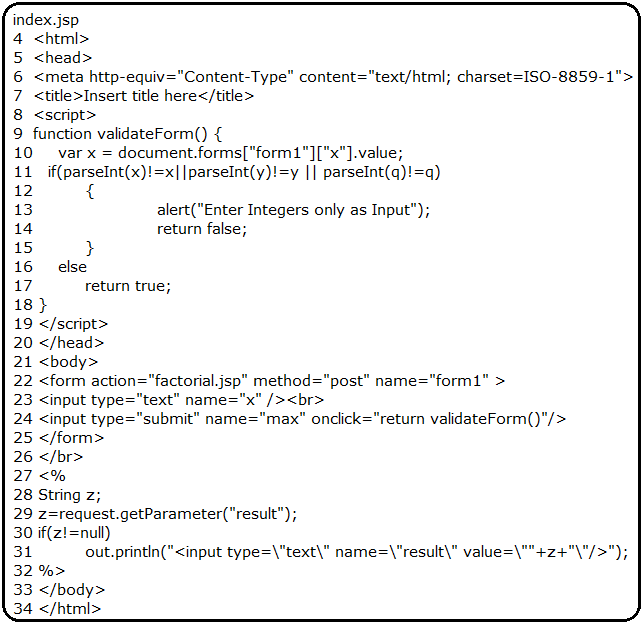
\includegraphics[scale=1]{index_l.png}
\caption{Example JSP program}
\label{fig3}
\end{center}
\end{figure}


\begin{figure}
\begin{center}
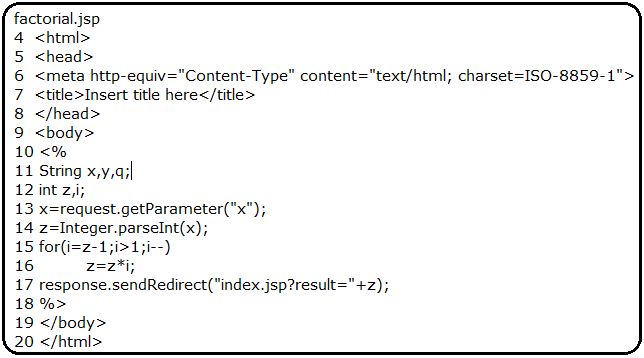
\includegraphics[scale=1]{factorial_l.png}
\caption{JSP program for calculating factorial of a number}
\label{fig4}
\end{center}
\end{figure}


\begin{figure}
\begin{center}
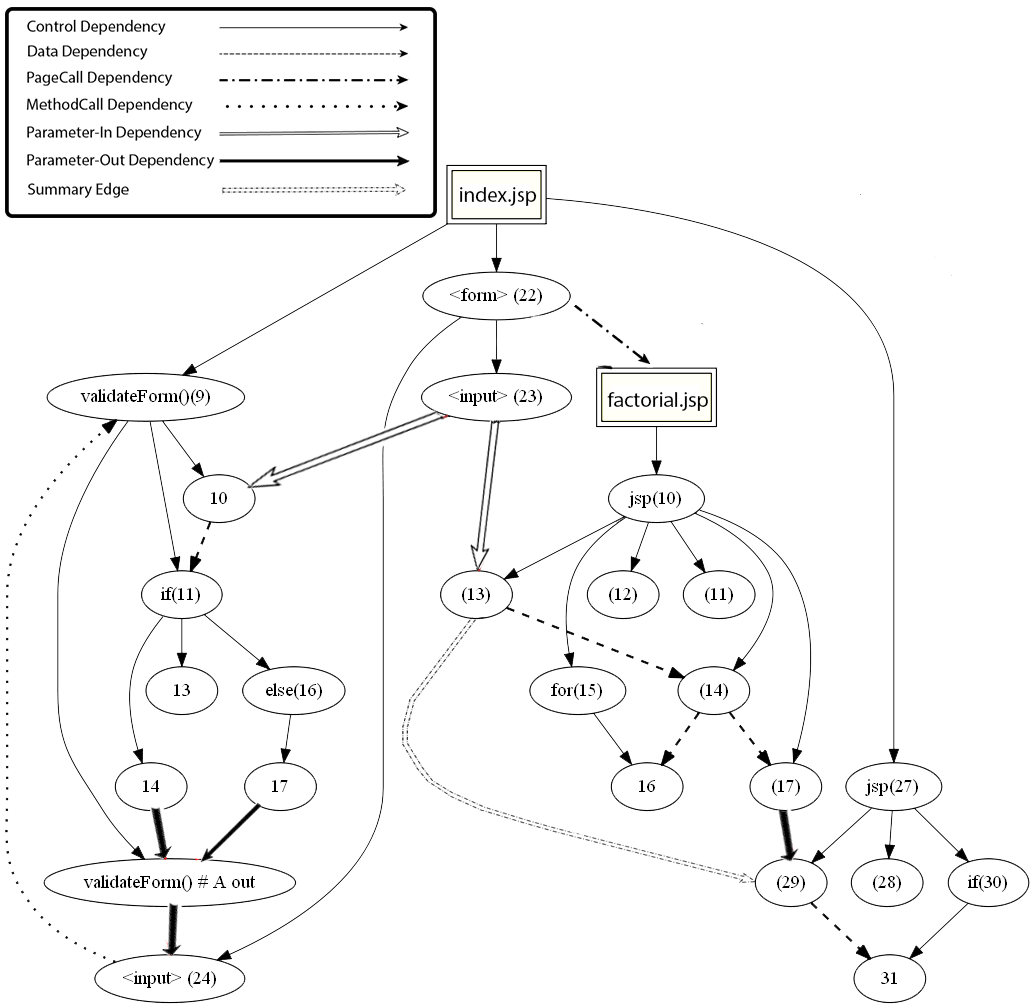
\includegraphics[scale=.5]{sdg_ll.png}
\caption{Generated WADG for the example programs in fig-\ref{fig3} and fig-\ref{fig4} }
\label{fig5}
\end{center}
\end{figure}

\subsection{WADG for dynamic code}
The problem of statically determining the HTML code generated dynamically by a Web application is in general undecidable. Consequently, it is in general impossible to build an accurate SDG for a Web application that generates some HTML code at run time.
Since it is not possible to determine the HTML code generated by a dynamic scripts in the general case, the typical patterns of code generation are considered and a technique to handle them is presented.

\subsubsection{Code Extrusion}
A JSP page may contain print statements which prints HTML code. In such cases, the output of such HTML code can only be know at runtime making it impossible to generate the WADG  with simple source code analysis.
To deal with this, we propose an algorithm of code extrusion, which converts and replaces the print statements with their HTML output in the source code.

\begin{algorithm}
\caption{CodeExtrusion}
\begin{algorithmic}[1]
\State \textbf{If} line contains “System.out.println”:\\
\hspace{2cm}a. Replace the print statement with an unquoted version of the printed string\\
\hspace{2cm}b. Replace concatenated variables with a print within JSP delimiters ($<$\% \%$>$). \\
\hspace{2cm}c. Call htmlParse(line).\\
\hspace{2cm}d. Add build dependency between print statement and generated HTML statement.
\end{algorithmic}
\end{algorithm}

\subsubsection{String-Cat Propagation}
A JSP page may contain variables initialized and concatenated with values which result in those variables containing HTML code. When print statements print such variables the same problem of dynamic code generation occurs as discussed in previous section, but cannot be resolved by code extrusion alone.
To deal with this, we propose an algorithm of string-cat propagation, which converts and replaces the print statements with the values of variables, containing HTML code, in the source code.
\begin{algorithm}
\caption{StringCatPropagation}
\begin{algorithmic}[1]
\State Create global HashMap strMap.
\State \textbf{if} line is a string assignment:\\
\hspace{2cm}a. Create a new entry in strMap with variable name as key and assigned string as value.
\State \textbf{else if} line is a string concatenation:\\
\hspace{2cm}a. Update strMap with new value of string.
\State \textbf{else if} line contains “System.out.print”:
\State \hspace{2cm} \textbf{if} argument of print contains variable from strMap:\\
\hspace{4cm}i. Replace variable with corresponding value from strMap.\\
\hspace{4cm}ii. codeExtrusion(line).
\State \hspace{2cm} \textbf{Else}\\
\hspace{4cm}i.	codeExtrusion(line).

\end{algorithmic}
\end{algorithm}
\subsubsection{Flow Information}
It might happen that a given JSP variable is associated to more than one string-cat after flow propagation. This occurs, for example, when alternatives are in the code(such as If Else construct).
To deal with this, we propose an algorithm of flow information , which converts and replaces the print statements with an $<$ALT$><$CASE$>$ HTML construct.
In the presence of loops,an $<$ALT$><$CASE$>$ construct with k(properly set) iterations is considered.

\begin{algorithm}
\caption{FlowInformation}
\begin{algorithmic}[1]
\State Create global HashMap altMap.
\State \textbf{if} line conatins if or line conatins else:\\
\hspace{2cm}a. Create multiple value entry in altMap with variable name as key and values from if and else.
\State \textbf{else if} line conatains loop:\\
\hspace{2cm}a. Create multiple value entry in altMap with variable name as key and values from k iterations.
\State \textbf{else if} line contains “System.out.print”:
\State \hspace{2cm} \textbf{if} argument of print contains variable from altMap:\\
\hspace{4cm}i. Replace print statement with $<$ALT$><$CASE$>$ construct using values from altMap.\\
\hspace{4cm}ii. codeExtrusion(line).

\end{algorithmic}
\end{algorithm}
\section{Slicing Algorithm}



\begin{algorithm}
 
 \caption{Slicing Algorithm : Two Phase}
 
 \textit{INPUT:} G- A WADG, s- Slicing Criterion, \\
 
 \textit{OUTPUT:} The Slice $S$ for $s$.\\
 lists and the result set
 
 \begin{algorithmic}[1]
  \State \hspace{1cm}W1 =\{s\}, W2 = \{\}, S =\{s\} //two work lists and the result set
  
 /* phase 1 */ 
 
 \State \textbf{repeat}
 
 \State \hspace{1cm}W1 =W1/ \{n\} // process the next node in W1 

 \State \hspace{1cm}\textbf{for all} $m -> _{e} n$ // handle all incoming edges of n 
 
 \State \hspace{2cm}\textbf{if} $m \notin S$ // m has not been visited yet 
 
 \State \hspace{3cm}S = $S\cup\{m\}$ // if e is not a param-out edge, add m to W1, otherwise, add m to W2 \\
 \hspace{4cm}\textbf{if} $e \notin \{po\}$ \\
 \hspace{5cm}$W1 =W1 \cup \{m\}$\\
 \hspace{4cm}\textbf{else} \\
 \hspace{5cm}$W2 =W2 \cup \{m\}$\\
 \hspace{1cm}$\textbf{Until W1} = \emptyset$
 
  /* phase 2 */ 
  
 \State \textbf{repeat}
 \State \hspace{1cm}W2 =W2/ \{n\} // process the next node in W2 
 \State \hspace{1cm}\textbf{for all} $m -> _{e} n$ // handle all incoming edges of n\\
 \hspace{2cm}\textbf{if} $e \notin \{pi,call\}$\\
 \hspace{5cm}$W2 =W2 \cup \{m\}$\\
 \hspace{5cm}$S =S \cup \{m\}$\\
 \hspace{1cm}$\textbf{Until W2} = \emptyset$\\
  \hspace{1cm}\textbf{return S}\\
  
 \end{algorithmic}
 
\end{algorithm}

After the construction of WADG for a given JSP program, we have to compute slices by taking different slicing criteria. We have used a two-phase slicing algorithm \cite{horwitz1990interprocedural}, as shown in Algorithm-2, for our slice computation.  Slicing as described in previous section is the process of selecting statements from the given web application with respect to an information of interest(slicing criterion) that replicates a part of the application itself. Sticking to this definition, Algorithm 2 takes an WADG of the web application and a slicing criterion as input, and gives a selected set of nodes from the WADG called slice as output. It performs the slicing operation in 2 phases, hence the name. The Algorithm recursively marks nodes of the WADG, starting with the slicing criterion itself, then proceeding to all its incoming edges. 

In the first phase, all edges except parameter-out edges are considered for marking.In the second phase, the parameter-out edges left in phase one are considered separately. This is done in order to avoid some undesirable nodes from being marked, as they are unrelated to the slicing criterion and should not be marked. As seen from the phase two of the algorithm, all the parameter-in and call edges are ignored and not added to slice.Think of this like a portion of code in one page gives an output which gets received and stored at some statement(say ST) of some other page. Now, in this situation, that particular portion of code has absolutely no relation with any other code which calls ST or gives an output to ST, hence should not be included in the slice, as achieved by the second phase of the algorithm.

To explain the working of the slicing algorithm, we have used the same example WADG shown in Figure-\ref{fig5}. Suppose the slicing criterion for this example is $s=31$. By using the slicing algorithm we have computed slice and shown it in Figure-\ref{fig6}. Here in this figure, the nodes included in the slice is shown as shaded nodes.



\begin{figure}
\begin{center}
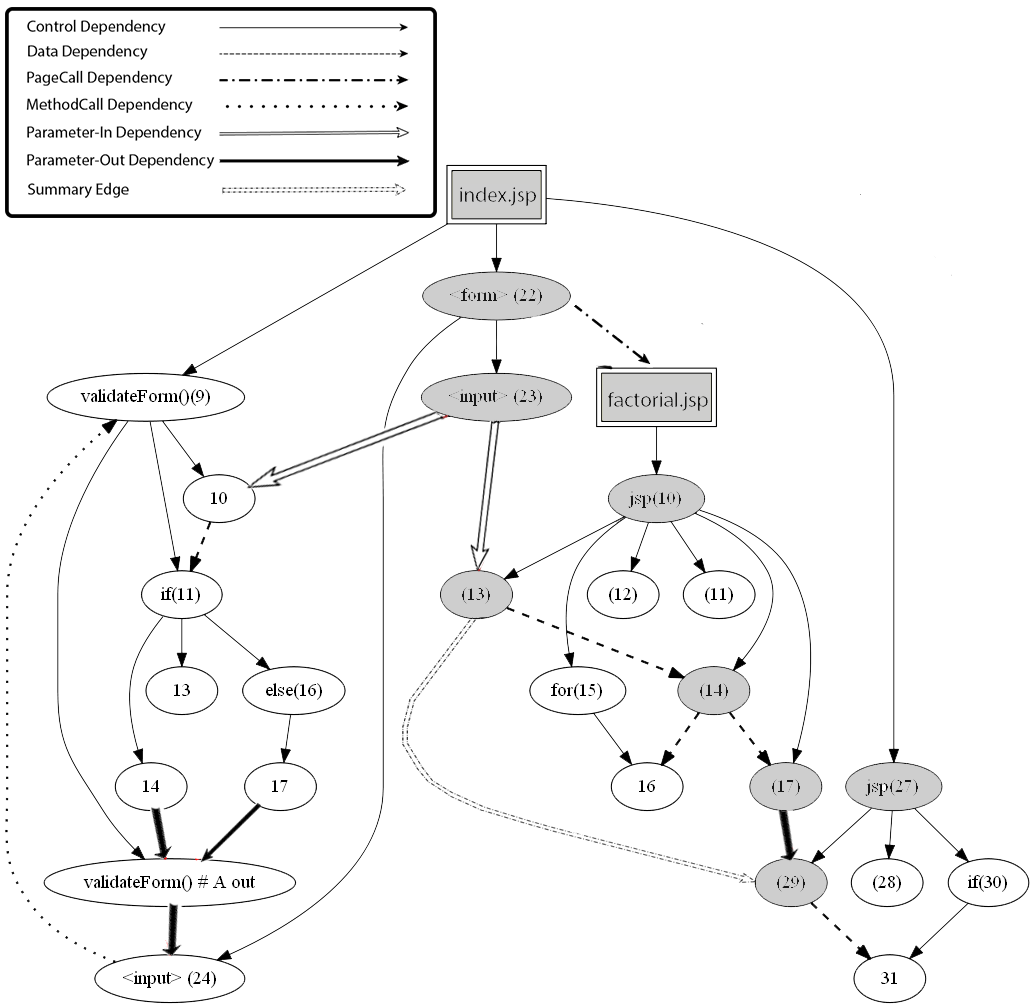
\includegraphics[scale=.5]{slice_ll.png}
\caption{Generated slice for WADG in fig-\ref{fig5} w.r.t. $s=31$}
\label{fig6}
\end{center}
\end{figure}

\section{Experimental Study}

We have developed a partial tool for automatic generation of WADG for a given JSP program. In the following section we are presenting the detailled implementation of our tool. Later, we have taken some real case studies to validate the working of our developed tool and slicing algorithm. We have performed the case studies with a personal computer having Intel Core $i5$ processor, clock speed 2.40GHz, primary memory 4 GB and Windows 7 Home Basic (64 bit) operating system.   

\subsection{Experimental Setup}

\begin{figure}
\begin{center}
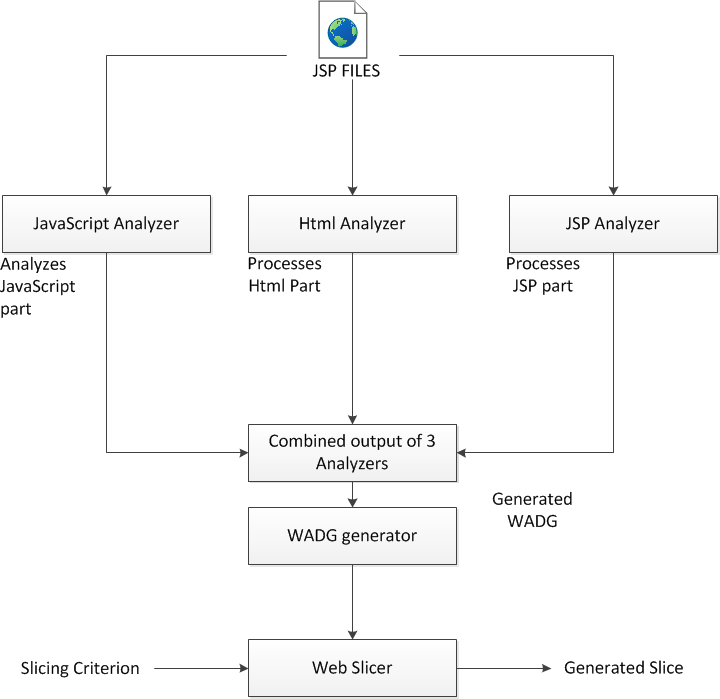
\includegraphics[scale=.8]{sdgflowchart.png}
\caption{A systematic block diagram for WebSlicer}
\label{fig7}
\end{center}
\end{figure}

In the block diagram, shown in Figure-\ref{fig7}, there are six sections that reads and analyzes each and every file of the web application sequentially and generates the WADG.\\At first the file is processed by JavaScript Analyzer that finds all the function names and variables names and stores them in different hash maps in key value pair. It also computes control and data dependence between JavaScript statements and sends results to the combined output section.

In the next section, HTML analyzer looks for two tags, i.e,$<input>$ and $<form>$ tags. If they contain any JavaScript function calls, a call dependency is added between them and matching nodes of the function map generated by the JavaScript section. If that function contains parameters, then a param-in dependence is added between nodes from HTMLmap and JSMap. Moreover, it computes control dependence between nodes and sends the results to the combined output section.


Finally, JSP analyzer process the JSP part. Control and data dependence between nodes is computed followed by a check for param-in dependence by checking the methods. Furthermore, it also checks if a page returns any parameter from which it was called and adds param-out dependence. The total processed result is sent to the combined output section of 3 analyzers. In the combined output of 3 sections, page call dependence is added between pages by checking the entry of the hash map provided by HTML section. Then it gives its output to the WADG generator section.

The WADG generator section receives the output of the previous sections and generates the WADG by writing a .gv file in the system. It adds all the dependencies according to the .gv file and also provides different dependencies by different notations. It generates the WADG completely and it gives its output to the WebSlicer. The WebSlicer receives the generated WADG file and the slicing criterion as input. Then, it process the WADG file and finds the node given by the slicing criterion. Finally, it generates the sliced WADG by applying the slicing algorithm on the input WADG and writes it to a .gv file in which the sliced nodes are marked.

\subsection{Case Study}

In-order to verify the ability of our designed WebSlicer tool, we have preformed three case studies. In each case study, we have taken one JSP program, then generated it's WADG. After that we have computed slices for the same program and WADG, by taking different slicing criteria. Choosing of slicing criteria is a difficult task, but we have fixed the output statements, like print statement or method return statements, as slicing criteria. The details of case studies is givien in Table-1. 

\begin{table}[htb]
 \centering
  \caption{Case study of various applications}
\label{tab1}
{ 
 \begin{tabular}{|p{.4cm}|l|l|}
 \hline  \bf{Sl. No.} & \bf{Name of Application}& \bf{Details}\\
 \hline  {1} & {Calculator} & {Performs mathematical operations} \\
 \hline  {2} & {Book Management System} & {Storage and issue of text books for an institute} \\
\hline  {3} & {Java EE Training} & {Tutorials and practice questions of Java} \\     
 \hline         
          \end{tabular}
 }
 \end{table}


\subsection{Findings}
First we have generated the WADG for each JSP applications, and the details are given in Table-2. Then we have computed several slices by supplying different slicing criteria. To summarise our finding, we have calculated the average slice size, which is the addition of individual slice size and number of slices computed. Similarly, we have computed the average slicing time, which is required to compute slices. Table-3 consists of all these findings.

\begin{table}[htb]
 \centering
  \caption{Details of generated WADG for case studies}
\label{tab1}
{ 
 \begin{tabular}{|l|l|p{3cm}|p{3cm}|p{3cm}|}
 \hline \bf{Name of Application}& \bf{LOC}& \bf{No Of nodes in WADG}& \bf{No Of Edges in WADG}& \bf{Time to Generate WADG} \\
 \hline  Calculator &  250 & 130 & 149 & 31.07 ms\\
 \hline  Book Management System &  834 & 527 & 612 & 114.39 ms\\
 \hline  Java EE Training  &  435 & 281 & 288 & 54.57 ms\\
  \hline   
          \end{tabular}
 }\end{table} 
 

 \begin{table}[htb]
 \centering
  \caption{Outcome of the case studies}
\label{tab1}
{ 
 \begin{tabular}{|l|l|l|l|}
 \hline  \bf{Sl. No.} & \bf{Name of Application}& \bf{Average Slice Size}& \bf{Average Slice Time}\\
     \hline  {1} & {Calculator} & {7} & {2.61 ms}\\
     \hline  {2} & {Book Management System} & {24} & {5.83 ms}\\
     \hline  {3} & {Java EE Training} & {18} & {3.17 ms}\\
  \hline   
          \end{tabular}
 }
 \end{table}

\section{Conclusion \& Future Work}
In this thesis, we have proposed a technique for slicing
of JSP programs. Most of the existing techniques are based on byte-code analysis of the program, which causes more
complex SDGs to represent and design. In our approach, we
have used the source-code based program analysis for construction of the WADG for a given JSP program. We have applied a two-phase slicing algorithm to compute slices. Then to verify our developed tool, we have conducted some case studies. The slices computed by our tool is check manually to be correct. We have found that all the slices computed by our technique is precise and correct. This technique can be further enhanced and used for dynamic slicing and   regression testing of web applications.

\bibliographystyle{unsrt}
\bibliography{Reference}

\end{document}